\chapter{Modelli}
\section{Automi cellulari}
Gli automi cellulari possono riprodurre fenomeni di auto-riproduzione e
auto-organizzazione, sono utili per modellare sistemi complessi dinamici e la
simulazione. Utili per simulare e studiare sistemi come: traffico, afflusso di
persone, percolazione (studio della fluido dinamica), sistema immunitario, sistemi
sociali etc\dots.

L'idea è di non descrivere il sistema complesso dall'alto, ad alto livello usando
sistemi di equazione differenziali. In realtà lo si fa simulando l'interazione
tra le celle, ognuna delle quali è definita attraverso una serie di regole locali
semplici.

Gli automi cellulari sono dei sistemi dinamici e discreti, dove i termini
rappresentano:
\begin{itemize}
    \item \textbf{Sistemi}: insieme di entità che interagiscono.
    \item \textbf{Dinamici}: evolvono nel tempo in un insieme di passi.
    \item \textbf{Discreti}: spazio, tempo e proprietà devono essere solo finiti
          con un numero numerabile di stati. Spazio finito perché dobbiamo
          rappresentare la realtà.
\end{itemize}
Esistono automi cellulari a più dimensioni che specificano quante dimensioni è lo
spazio.

Lo spazio su cui essi operano è rappresentato da una griglia di celle discrete.
Inoltre, si ha un tempo di evoluzione discreto.

Lo stato che ogni cella assume è definito a partire da un insieme finito di stati
possibili. Inoltre, l'evoluzione di ogni cella è determinata da una regola comune
per tutte le celle, e dipende solamente dallo stato attuale della cella e dagli
stati dei suoi vicini. La regola di aggiornamento è quindi locale e uniforme.
\begin{definizione}[\textbf{Automa cellulare}]
    Un \textbf{automa cellulare} è definito come una tupla:
    \begin{equation*}
        \langle L, Q, q_0, u,f\rangle
    \end{equation*}
    dove:
    \begin{itemize}
        \item $L$: è l'array di automi a stati finiti uniformi.
        \item $Q$: insieme di stati finiti.
        \item $q_0$: è lo stato iniziale.
        \item $u$: è una funzione che definisce il criterio di connessione della
              singola cella con quelle adiacenti.
              \begin{equation*}
                  u: L \rightarrow L^{k}
              \end{equation*}
        \item $f$: la regola di transizione locale.
              \begin{equation*}
                  f: Q^{k} \rightarrow Q
              \end{equation*}
    \end{itemize}
\end{definizione}
Lavorando con automi cellulari finiti, ovvero con lo spazio finito, sarà
importante definire una \textbf{condizione di bordo}, ovvero come deve essere la
regola del vicinato quando le celle sono vicino al bordo. La scelta della
condizione di bordo può essere fatta in questo modo:
\begin{itemize}
    \item Collegare i bordi: i bordi opposti dello spazio sono collegati. Si crea
          quindi un ambiente toroidale.
    \item Guardare i bordi come uno specchio: si considera che il bordo sia uno
          specchio, quindi si riflette il contenuto della cella.
\end{itemize}
Per gli automi cellulari 1-D in cui gli stati delle celle sono binari, si possono
codificare le regole attraverso numeri decimali.

Per mostrare l'evoluzione dell'automa 1D si usa il diagramma spazio-tempo, dove
si mostra l'evoluzione dell'automa nel tempo.
\begin{esempio}[Traffico]
    La regola del traffico è rappresentata dal valore 184. Essa permette di
    modellare semplicemente il flusso del traffico su una strada a singola corsia.

    La rappresentazione del traffico avviene nel seguente modo:
    \begin{figure}[!ht]
        \centering
        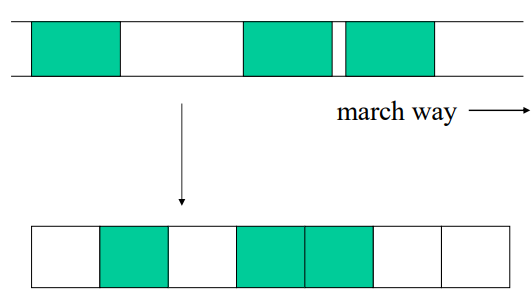
\includegraphics[width=0.5\textwidth]{./img/modelli/ese_traffico.png}
        \caption{Esempio di automa cellulare per la rappresentazione del traffico.}
        \label{fig:ese_traffico}
    \end{figure}
    La regola 184 è definita come segue:
    \begin{itemize}
        \item 111: il veicolo rimane fermo (1)
        \item 110: il veicolo si sposta in avanti e quindi la cella rimane vuota
              (0)
        \item 101: la cella è vuota e quindi il veicolo a sinistra si sposta
              occupando la cella (1)
        \item 100: la cella è vuota e quindi il veicolo a sinistra si sposta
              occupando la cella (1)
        \item 011: la cella a destra è occupata quindi il veicolo rimane fermo
              (1)
        \item 010: la cella a destra è vuota e quindi il veicolo si sposta in
              avanti (0)
        \item 001: non ci sono veicoli nella cella attuale e nella precedente
              quindi resta vuota (0)
        \item 000: non ci sono veicoli la cella è vuota (0)
    \end{itemize}

    Questo modello non rappresenta la realtà, in quanto ogni macchina si muove a
    step di 1 se c'è spazio, altrimenti si ferma. Inoltre, non si considera il
    tempo di reazione del guidatore e molti altri fattori.

    Possiamo complicare leggermente il modello sostituendo il valore che 
    rappresenta la presenza o meno del veicolo con la velocità del veicolo.
    Si aumenta il raggio delle celle da considerare come vicine. Inoltre, ogni 
    veicolo accelera di una velocità fino a quando non rischia di fare incidenti.
\end{esempio}

\begin{nota}
    Le celle possono essere anche triangolari, esagonali e pentagonali. Infatti 
    spesso si usano gli esagoni al posto dei quadrati, perché permettono di mantenere
    la velocità di spostamento degli elementi uguale anche in diagonale. Il vicinato 
    ad esagono si implementa con 3 vicini da una parte e 3 vicini dall'altra.
\end{nota}

Per gli automi cellulari sarà importante definire un raggio del vicinato, estendere 
il raggio permette alle celle di essere influenzate da celle presenti nel vicinato,
istantaneamente senza attendere il tempo per raggiungere la cella. Estendere il 
raggio, implica maggior complessità.

\begin{nota}
    Non abusare dei termini per la relazione, ex: emergenza di un fenomeno.    
\end{nota}

Esistono automi che sono invarianti secondo la rotazione, in generale sono 
quelli che effettuano un conto sui vicini, inoltre non hanno una direzione dei vicini. 
Questi automi sono detti totalitaristici.

\section{Modellazione della folla di persone}
Inizialmente la modellazione delle folle di persone è stata effettuata considerando 
le singole persone senza relazioni tra di loro quindi:
\begin{itemize}
    \item Ogni persona ha un proprio obiettivo
    \item Le altre persone sono considerate come ostacoli
\end{itemize}

Ora si vuole modellare la folla di persone con delle relazioni (Ex: madre-figlia,
gruppi di persone differenti). 

All'epoca non c'era molto, si è partiti da uno studio di architetti che hanno 
osservato un marciapiede e categorizzavano le persone che passavano su quel marciapiede 
e se fossero singole o a gruppi. Si è notato che i gruppi hanno velocità più bassa e 
una ridotta varianza nella velocità rispetto al singolo. Hanno fatto lo stesso 
studio è stato effettuato in un aereoporto e si è notato che le velocità medie e la varianza 
cambiano. Inoltre più aumenta la dimensione dei gruppi allora più bassa è la velocità
e più costante sarà. Si modella usando il social force model con una forza aggiuntiva 
che modella la formazione delle persone nei gruppi. (ex: Line-ABreast, V-like, River-like nei gruppi da 3).

Esistono anche modelli più complessi che non si limitano a gruppi piccoli, in realtà 
la moda dei gruppi è spesso $3$.

Studio della folla che passa in galleria: si è notato che i gruppi vanno da $1$ a $4$
persone, di cui i gruppi da $4$ sono molto piccoli. Si è notato che i singoli sono 
più veloci e hanno traiettorie meno lineari, mentre il contrario per i gruppi.

è stata successivamente studiata la dispersione, si è notato che gruppi piccoli
sono meno dispersi mentre gruppi più grandi si dispergono maggiormente. Studiato
il fenomeno reale è stato definito il modello, si è partiti dai sistemi 
dinamici discreti, si è partiti da \textbf{floor field CA}. Il modello 
è basasto su:
\begin{itemize}
    \item spostamento probabilistico
    \item goal oriented: abbiamo un gradiente che specifica la direzione dell'obiettivo
    \item presenza di ostacoli: simula gli ostacoli è statica
    \item presenza di altri pedoni: simula la folla che è dinamica si calcola ad 
    ogni passo. Si valuta negativamente perché si cerca di stare lontano.
\end{itemize}
è stato aggiunto:
\begin{itemize}
    \item nozione di gruppo: coesione del gruppo per modellare i gruppi che 
    rallenta le persone del gruppo se uno rallenta
\end{itemize}
la modellazione dell'ambiente è stata fatta discretizzandolo (introducendo un errore)
si hanno dei marker di inizio (generazione di agenti) e fine (obiettivo e distruzione di agenti). 

Per effettuare lo spostamento degli agenti si determina la metrica della distanza 
e questo implica l'induzione di particolari comportamenti. Inoltre è stata implementata 
la possibilità di occupare mezza cella aumentando la densità. Si è introdotta la 
coesione tra individui dello stess gruppi.

Si è notato che gli individui hanno una velocità più elevata quando aumenta la densità,
fino a quando è troppa e quindi diventano lenti quanto il singolo. Addirittura 
il flusso dei gruppi diventa superiore perché si mettono in coda.
Nell'osservazione reale si notava la dispersioen, questo può essere implementato 
nel modello sempre calcolando i centroidi e questo permette di testare l'algoritmo 
di coesione per confrontarlo nella realtà.

L'aggiornamento degli agenti si può effettuare:
\begin{itemize}
    \item sequential shuffle update: genero 
    una sequenza di pedoni randomica e aggiorno un pedone alla volta.
    \item parallel update: si sceglie il movimento per ogni pedone, si risolvono 
    i conflitti (uno si muove e l'altro no, altrimenti si fermano entrambi)    
\end{itemize} 
L'approccio basato sugli atuomi cellulari porta ad dei limiti, come le traiettorie 
zig-zag, in aggiunta dobbiamo simulare anche la velocità. Questo lo possiamo fare 
in base alla frequenza di aggiornamento, dimensione della cella e ottenere la 
velocità corrispondente nel mondo reale. Se abbiamo velocità diverse (eterogenee)
possiamo tranquillamente modificare quante volte si muovono per turno, il problema
è che ci potrebbe essere il problema di traiettorie che si intrecciano, quindi 
conflitti e anticiparli non è così banale.

Un'alternativa è considerare la velocità come numero reale tra $0-1$ al posto che 
il numero di celle.

C'è anche un meccanismo di Reaction Time.

I limiti del modello è che nello spazio possiamo avere corridoi obliqui e quindi 
compiamo degli errori nel modello e si può stimare l'errore. Questo è dovuto all'utilizzo
dei CA che discretizzano con celle. 

Se volessimo modellare le scale allora è come se le celle rallentano la velocità 
dell'individuo.

Successivamente si prende il modello e si compara con quanto osservato.